104. \begin{figure}[ht!]
\center{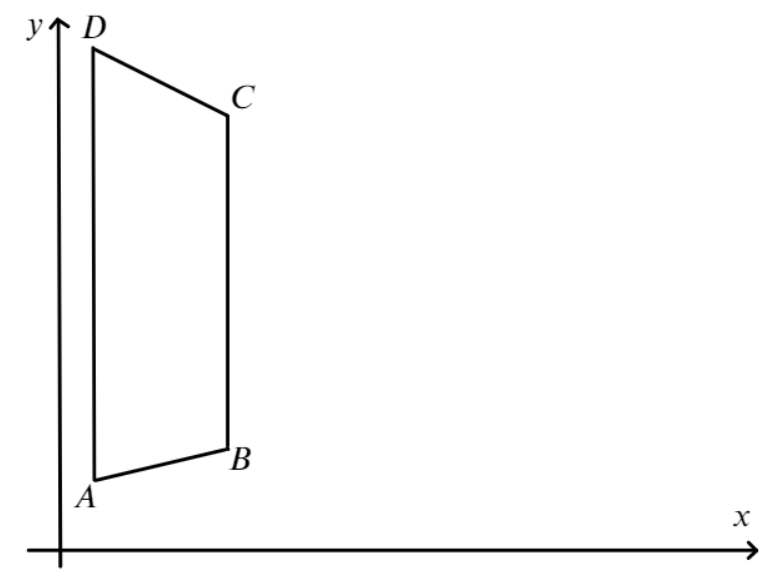
\includegraphics[scale=0.35]{g9-104.png}}
\end{figure}\\
Если трапеция вписанная, то она равнобедренная. Так как ордината точки $B$ на 1 больше ординаты точки $A,$ ордината точки $D$ должна быть на 1 больше ординаты точки $C,$ то есть $C$ имеет координаты $(5;17).$ Высота трапеции равна $5-1=4,$ значит $S_{ABCD}=4\cdot\cfrac{(18-2)+(17-3)}{2}=60.$\\
